% Fig. candidate for the method / recording setup: the camera on its rig, labelled.
% One column (3.5 in = 252 pt). Build: pdflatex rig.tex
\documentclass[tikz,border=1pt]{standalone}
\usepackage[T1]{fontenc}
\usepackage{newtxtext,newtxmath}
\usepackage{graphicx}
\usetikzlibrary{arrows.meta,calc}

\definecolor{ink}{HTML}{0B0B0B}
\definecolor{muted}{HTML}{52514E}

\tikzset{
  font=\footnotesize,
  call/.style={draw=ink, line width=0.5pt, -{Circle[length=2.2pt]}},
  lab/.style={align=left, anchor=west, inner sep=1pt, text=ink},
  sub/.style={font=\scriptsize\itshape, text=muted},
}

\begin{document}
\begin{tikzpicture}[x=1mm, y=1mm]
\node[anchor=south west, inner sep=0pt] (photo) at (0,0) {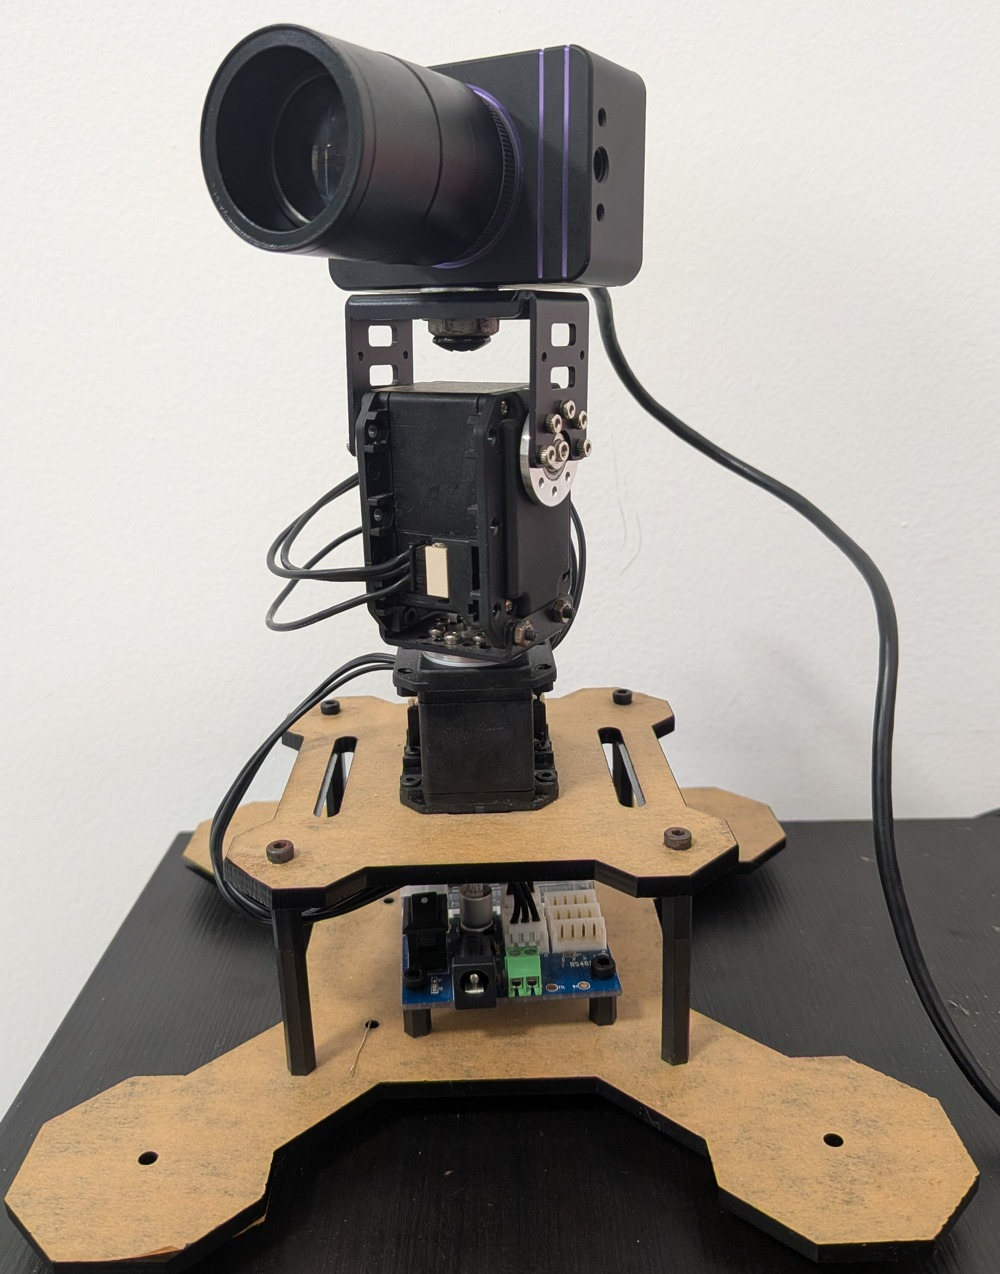
\includegraphics[height=58mm]{assets/rig.jpg}};
% photo is 1000 x 1274 px; positions below are fractions of its width and height
\coordinate (cam) at ($(photo.south west)+(0.43*45.53,0.87*58)$);
\coordinate (servo) at ($(photo.south west)+(0.46*45.53,0.61*58)$);
\coordinate (base) at ($(photo.south west)+(0.47*45.53,0.41*58)$);
\coordinate (board) at ($(photo.south west)+(0.51*45.53,0.25*58)$);

\node[lab] (l1) at (50,52) {\textbf{DVXplorer} event camera\\[-1pt]{\scriptsize\itshape\color{muted} 640\,$\times$\,480 pixels}};
\node[lab] (l2) at (50,36) {tilt servo};
\node[lab] (l3) at (50,26) {pan servo};
\node[lab] (l4) at (50,14) {servo driver};

\draw[call] (l1.west) -- (cam);
\draw[call] (l2.west) -- (servo);
\draw[call] (l3.west) -- (base);
\draw[call] (l4.west) -- (board);
\end{tikzpicture}
\end{document}
